\section*{Why Not Regularize $\theta_0$?}
        
        \begin{kequation}
            In general, our \vocab{regularizer for regression} will be given by \purp{square magnitude} of $\theta$:
            
            \begin{equation*}
                R(\Theta) = \norm{\theta}^2 = \theta \cdot \theta
            \end{equation*}
            
            This approach is called \vocab{Ridge Regression}.
        \end{kequation}
        
        \note{We'll discuss why it's called "ridge" regression once we find our solution.}
        
    \subsection*{Why not include $\theta_0$?}
    
        One thing you might immediately notice is that we used the magnitude of $\theta$ instead of $\Theta$: this omits $\theta_0$. Why would we do that?
        
        We'll show that we need to \textbf{allow} the \textbf{offset} to have whatever value works best, and we shouldn't \textbf{punish} it. 
        \note{For simplicity, we won't do any regularization here: we can make our point without it.}
        
        This is best shown with a \textbf{visual} example. Let's take an example with one input $x_1$. So, we have a \textbf{linear} function: \red{$h(x) = \theta_1x_1+\theta_0$}.
        
        \begin{figure}[H]
        \centering
            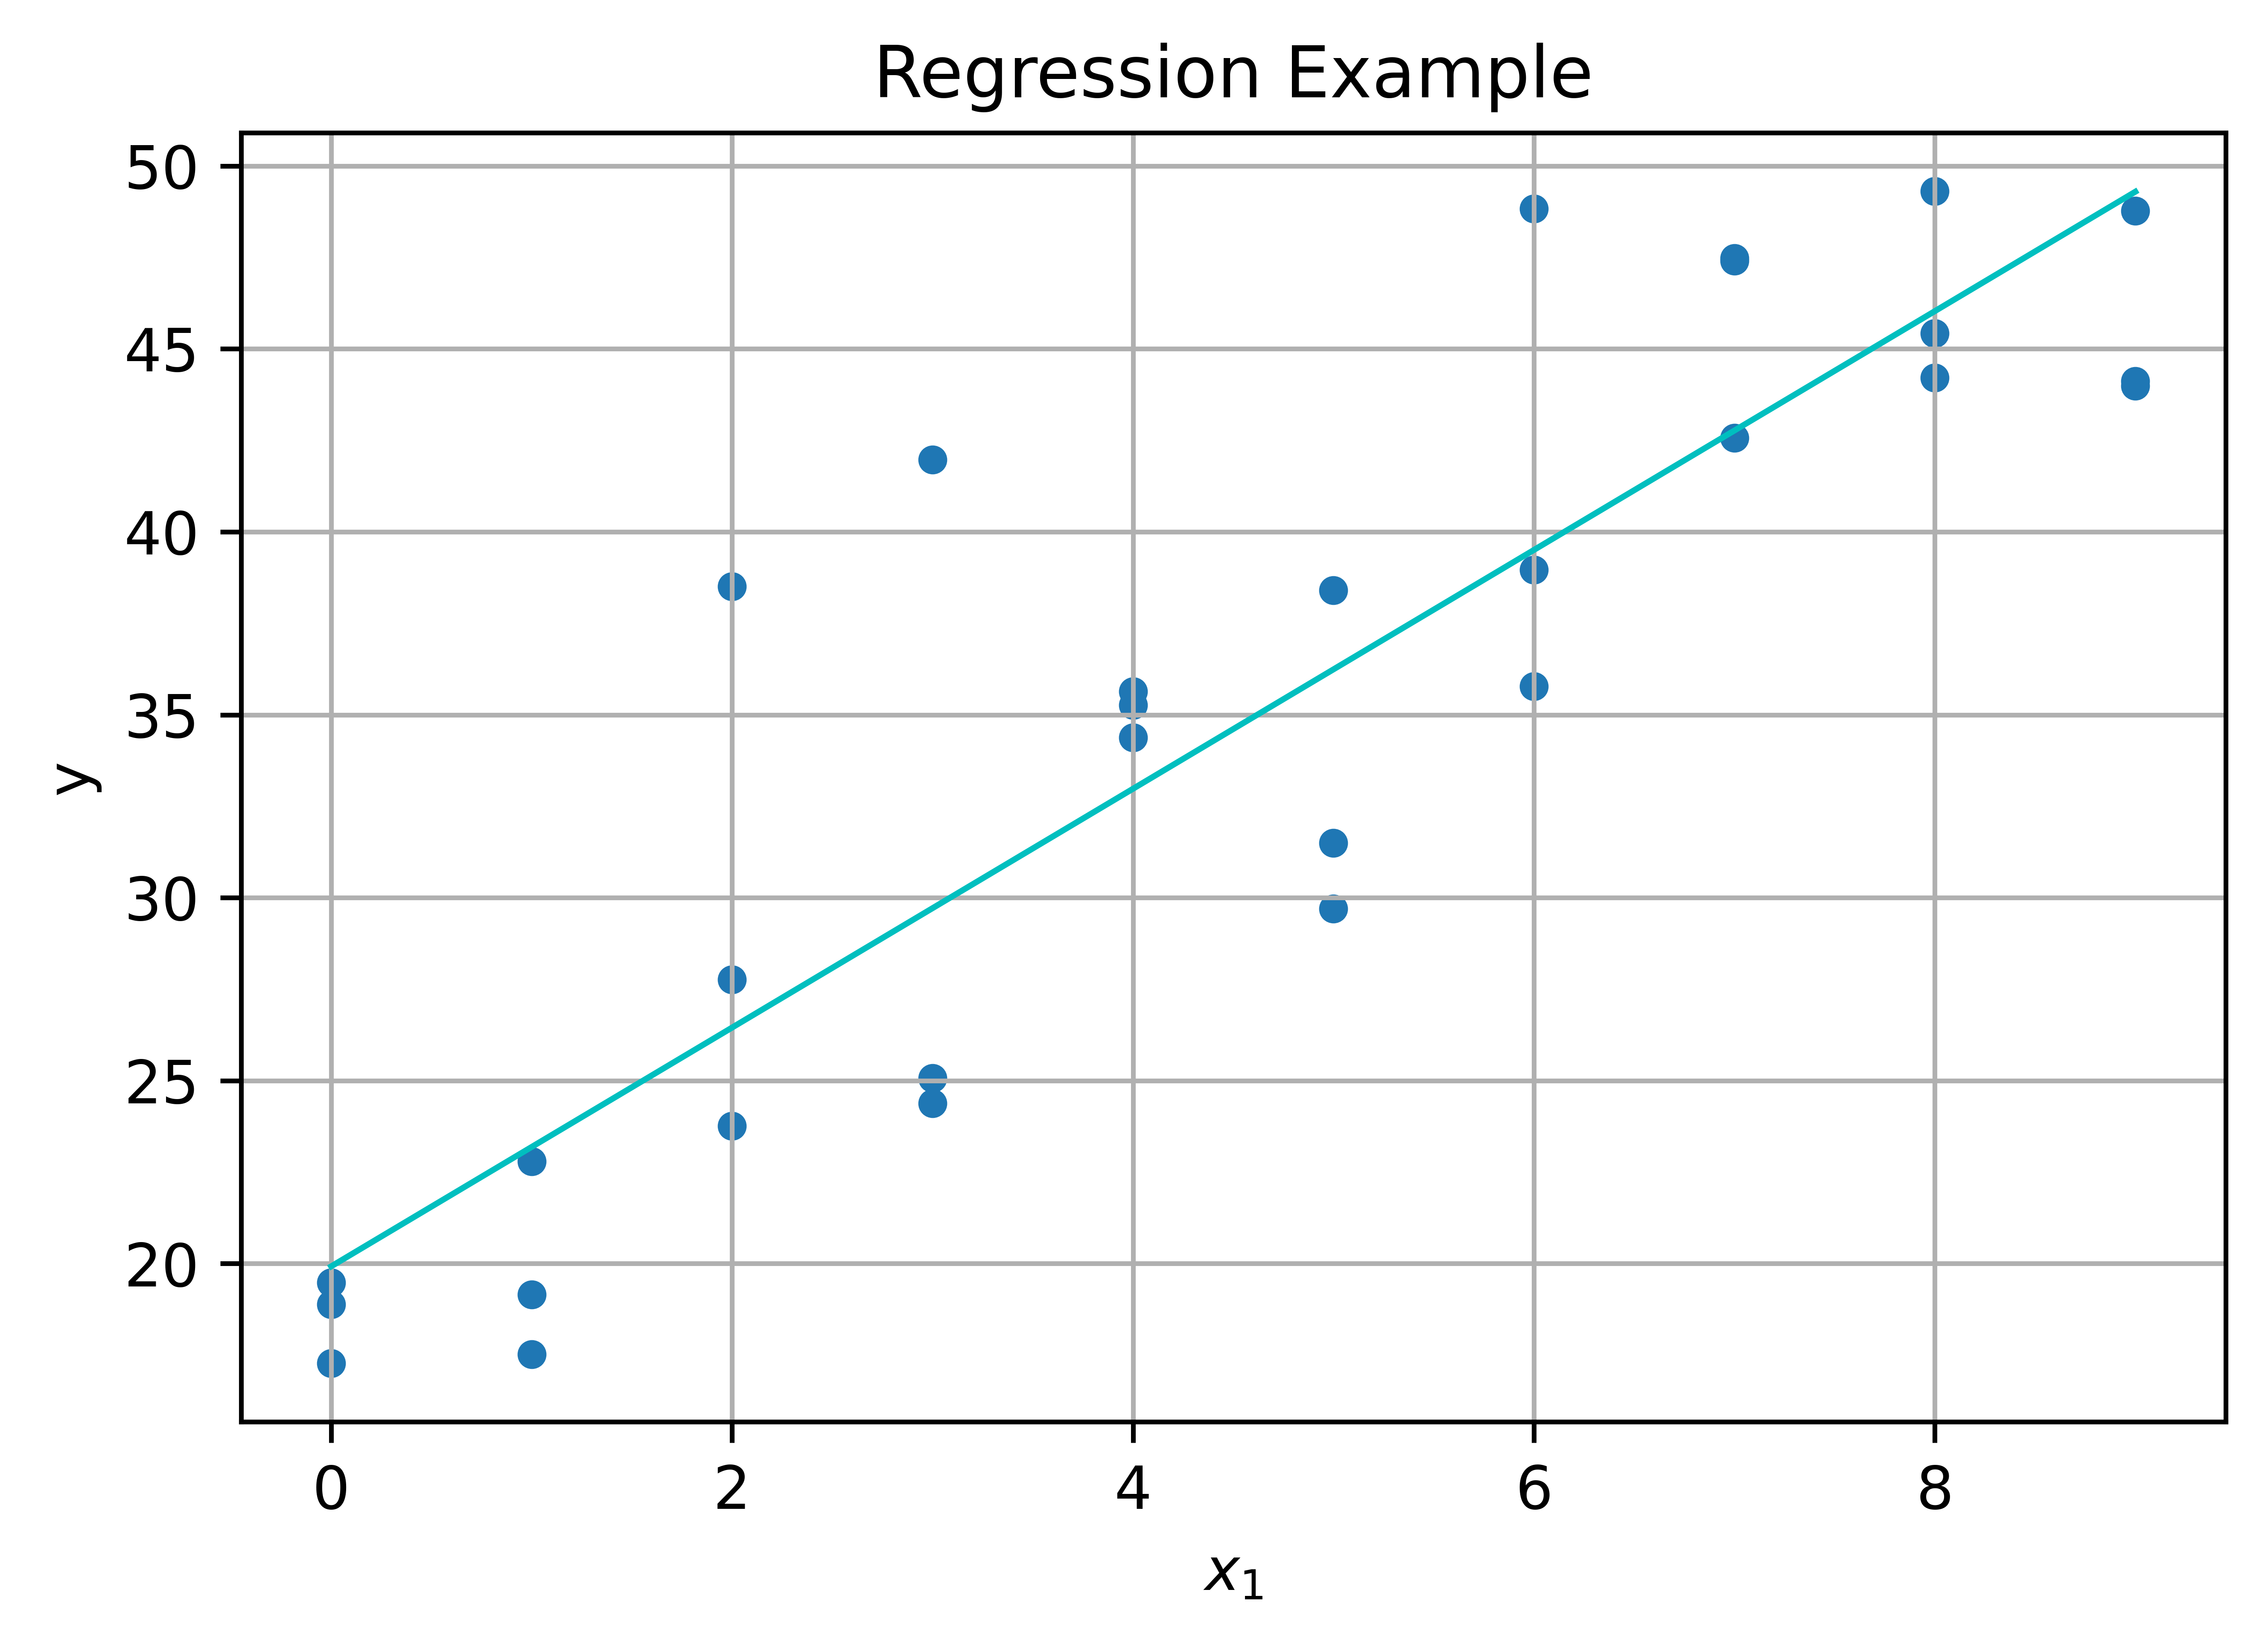
\includegraphics[width=70mm,scale=0.5]{images/regression_images/Regression_Keep_Offset.png}
        
            \caption*{Our regression example.}
        \end{figure}
        
        Let's suppose we \textbf{push} for a \textbf{much lower} (offset) $\theta_0$ term, while keeping everything else the \textbf{same}:
        
        \begin{figure}[H]
        \centering
            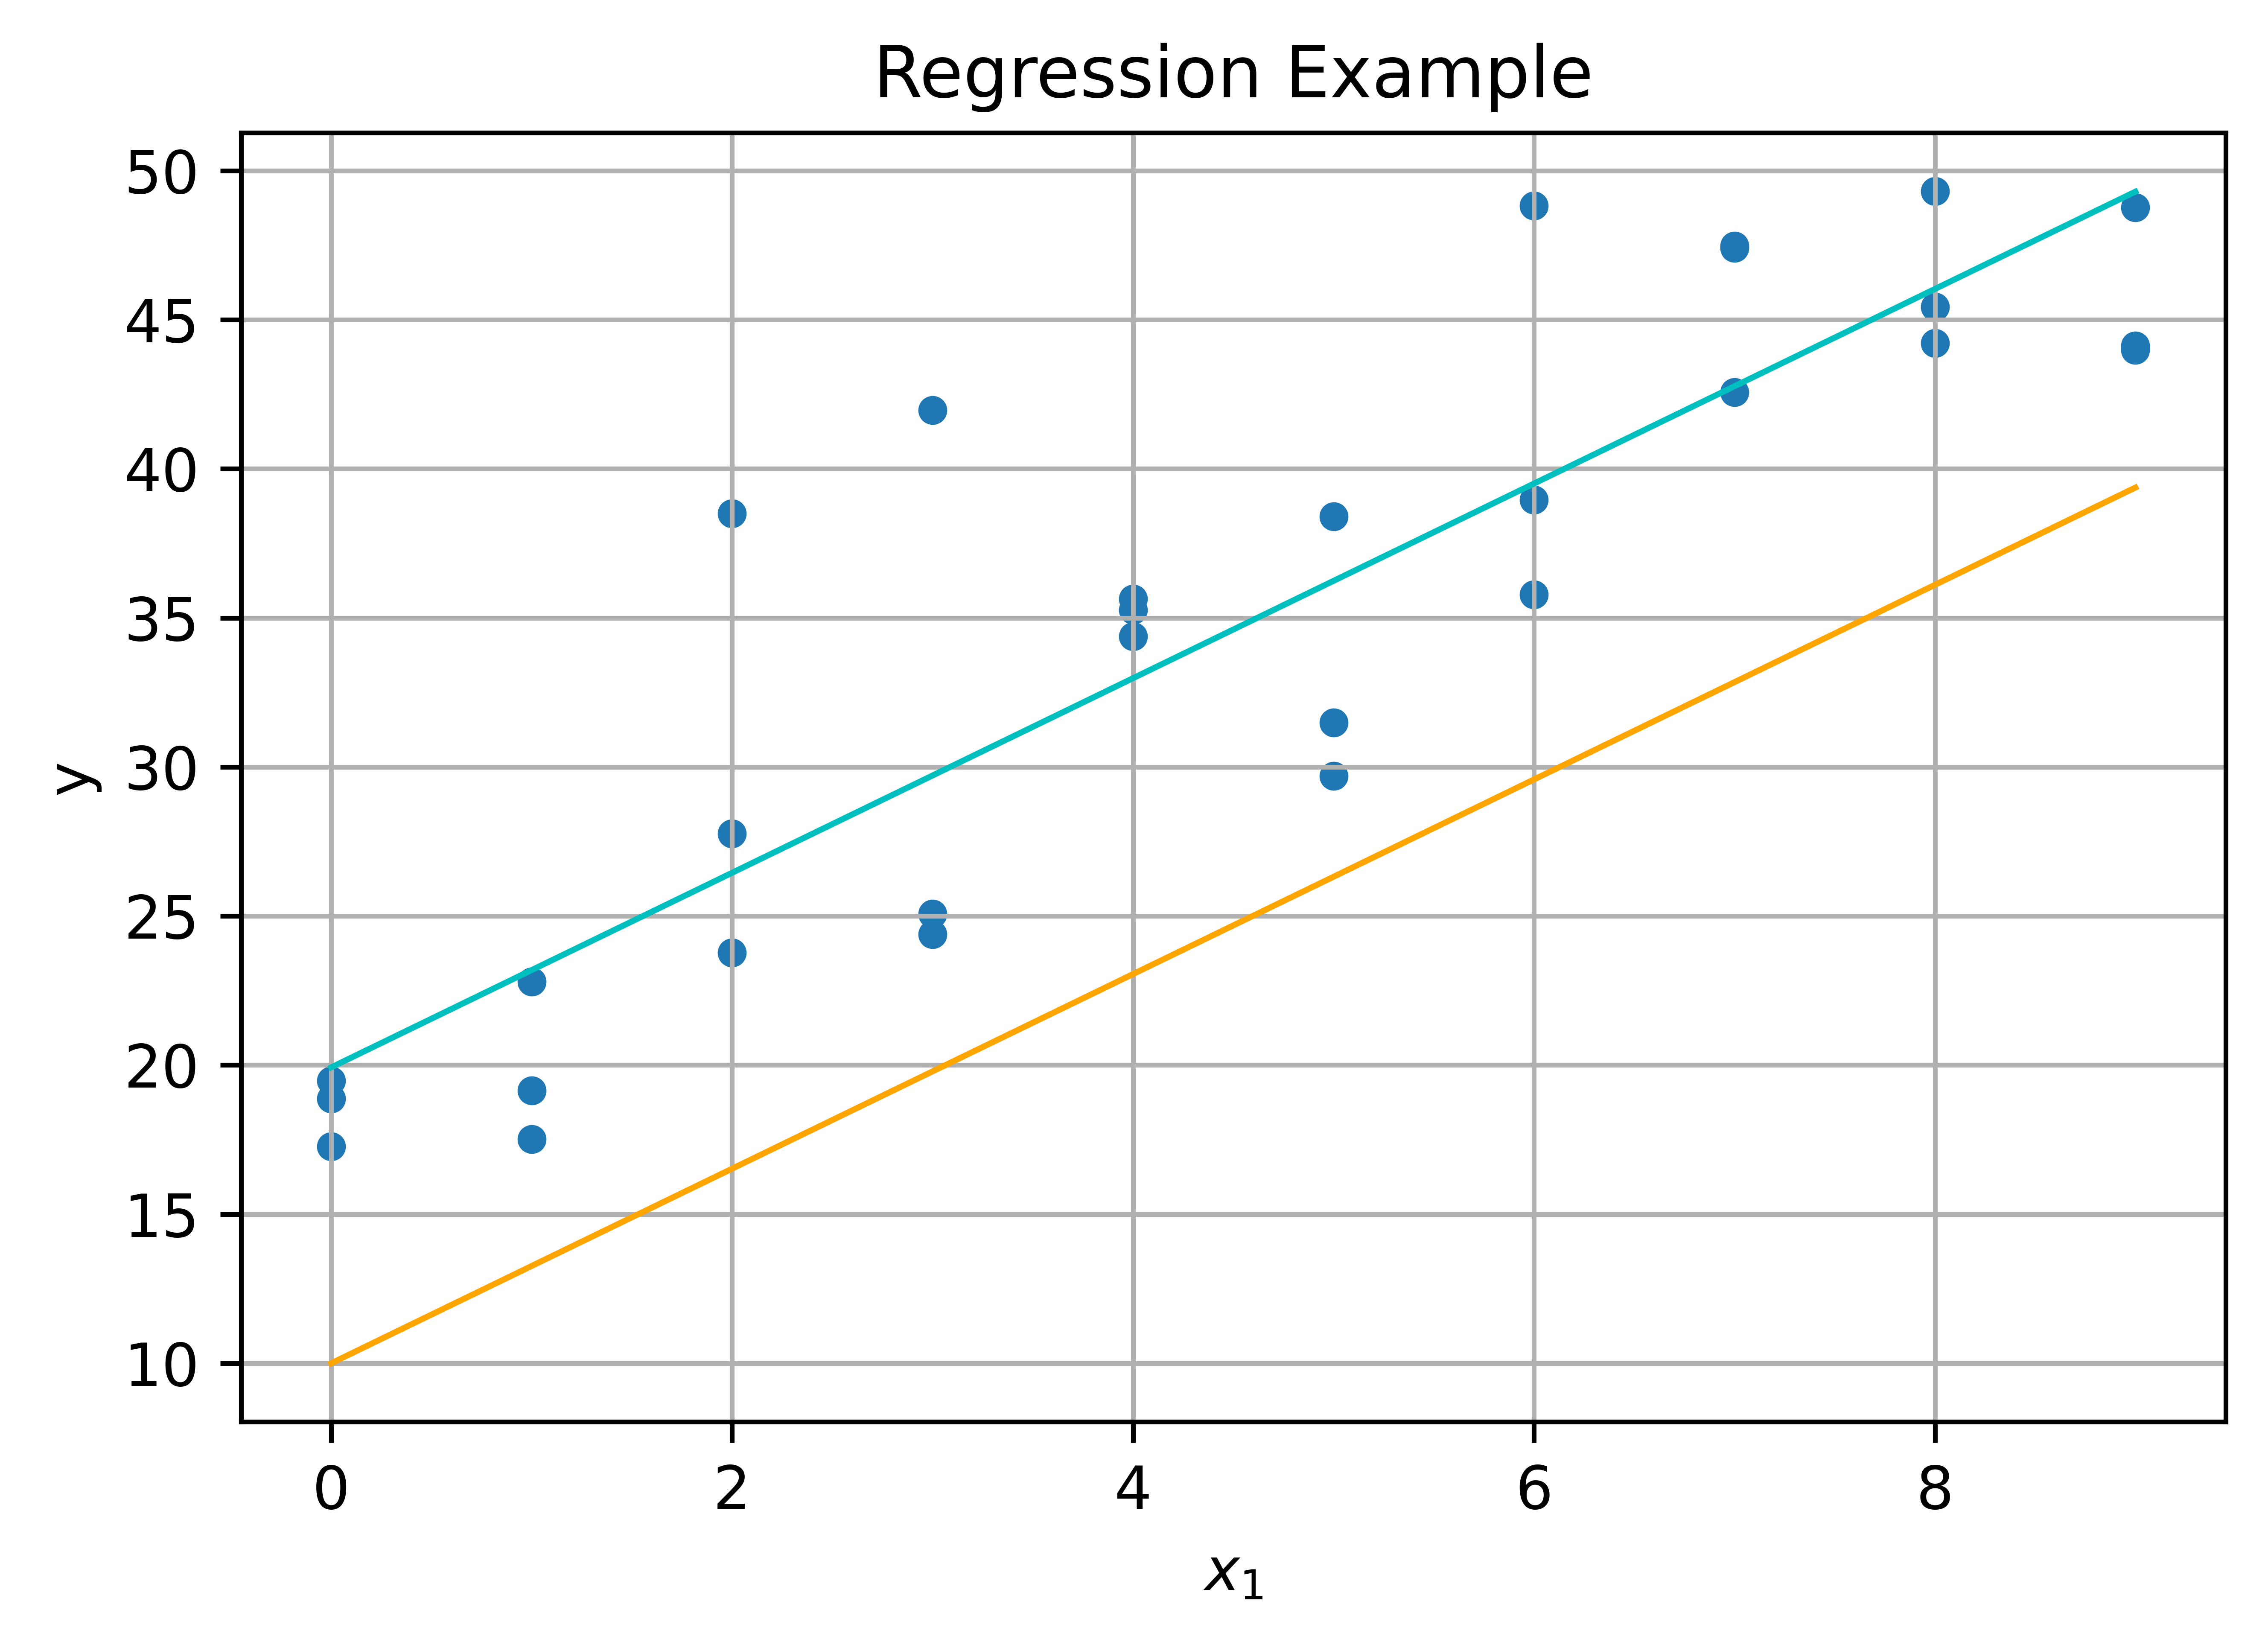
\includegraphics[width=70mm,scale=0.5]{images/regression_images/Regression_Remove_Offset.png}
        
            \caption*{Reducing our offset pulls our line further away from all of our data! That's not helpful.}
        \end{figure}
        \note{And regularizing $\theta_1$ wouldn't make this any better: it would just be flatter.}
        
        This shows that we \textbf{need} our offset! We use it to \textbf{slide} our hyperplane around the space: if all of our data is \textbf{far} from $(0,0)$, we need to be able to \textbf{move} our \textbf{entire line}.
        
        So, we'll keep $\theta_0$ \textbf{separate} and \textbf{allow} it to take whatever value is \textbf{best}.\\
        
        \begin{concept}
            We \purp{do not regularize} our \purp{offset} term, $\theta_0$. 
            
            Instead, we allow $\theta_0$ to \gren{shift} our hyperplane wherever it \gren{needs} to be.
        \end{concept}
        
        The other terms $\theta$ control the \textbf{orientation} of the hyperplane: the \textbf{direction} it is \textbf{facing}. We \textbf{regularize} this to push it towards less "complicated" orientations.
        \note{This will be discussed more in-depth in the Classification chapter!}

        
